% Created 2025-04-29 Tue 19:33
% Intended LaTeX compiler: pdflatex
\documentclass[11pt]{article}
\usepackage[utf8]{inputenc}
\usepackage[T1]{fontenc}
\usepackage{graphicx}
\usepackage{longtable}
\usepackage{wrapfig}
\usepackage{rotating}
\usepackage[normalem]{ulem}
\usepackage{amsmath}
\usepackage{amssymb}
\usepackage{capt-of}
\usepackage{hyperref}
\usepackage{minted}
\usepackage{siunitx, graphicx}
\graphicspath{ {./images/} }
\author{Hankertrix}
\date{\today}
\title{Introduction To Molecules Notes}
\hypersetup{
 pdfauthor={Hankertrix},
 pdftitle={Introduction To Molecules Notes},
 pdfkeywords={},
 pdfsubject={},
 pdfcreator={Emacs 30.1 (Org mode 9.7.11)}, 
 pdflang={English}}
\begin{document}

\maketitle
\setcounter{tocdepth}{2}
\tableofcontents \clearpage\section{Definitions}
\label{sec:orgbe197f7}

\subsection{Chemical bonds}
\label{sec:org77df3fe}
Chemical bonds are formed between atoms because the resulting compounds are more stable than the separate atoms. Examples of chemical bonds include ionic bonds, which are formed when the atoms gain or lose electrons, and covalent bonds, which are formed when the atoms share electrons.
\subsection{Lewis structures}
\label{sec:org48c6dae}
Lewis structures, also known as electron-dot structures, show the valence electrons of an atom as dots.
\subsection{Kekule structures}
\label{sec:org371b4cf}
Kekule structures, also known as line-bond structures, uses lines to indicate the bonds between atoms. A single line represents a two-electron covalent bond. The number of covalent bonds an atom forms \textbf{depends on how many valence electrons it needs to reach a noble-gas configuration}.
\subsection{Lone pair electrons}
\label{sec:org0c3c8b4}
Lone pair electrons are valence electrons that are not involved in bonding.
\subsection{Valence bond theory (orbital hybridisation)}
\label{sec:org6c8bc2a}
The valence bond theory is a model of chemical bonding to explain the placement of atoms in a molecule in 3D space.
\subsection{Bond polarity}
\label{sec:org8086dda}
Covalent bonds that have ionic character are known as polar bonds. This means that the electron distribution between the atoms involved in the covalent bond is not symmetrical and the bonding electrons are more strongly attracted by one atom.
\subsection{Electronegativity (EN)}
\label{sec:orgddeeb55}
Electronegativity is the intrinsic ability of an atom to attract the shared electrons in a covalent bond.
\subsection{Dipole moment (\(\mu\))}
\label{sec:orgdfd1263}
A dipole moment is the net molecular polarity due to the difference in summed charges.

\begin{itemize}
\item \(\mu\) is equal to the magnitude of charge \(Q\) at the end of the molecular dipole times the distance \(r\) between charges.
\item \(\mu = Q \times r\), in \emph{debyes} (\(D\)), \(\qty{1}{\unit{D}} = 3.336 \times 10^{-30} \text{ coulomb meter } (C \cdot m)\)
\end{itemize}
\subsubsection{Polar molecules}
\label{sec:orgfc9f2d8}
\begin{itemize}
\item The electronegativity of \(O\) and \(N\) is greater than that of \(H\).
\item Both \(O\) and \(N\) have lone-pair electrons oriented away from the nuclei, giving rise to a considerable charge separation and a \textbf{large dipole moment}.
\end{itemize}
\subsubsection{Non-polar molecules}
\label{sec:org972d7c5}
In symmetrical molecules, the dipole moment of each bond has one in the opposite direction, which cancels each other out, resulting in a net dipole moment of zero.
\subsection{Resonance}
\label{sec:orgc366b9e}
Resonance refers to the delocalisation of the \(\pi\) bond and lone pair electrons in the molecule.
\subsubsection{Rules for drawing resonance structures}
\label{sec:org3fd7d28}
\begin{enumerate}
\item Individual resonance forms are \textbf{imaginary}. The real structure is a hybrid.
\item Resonance forms differ only in the placement of their \(\pi\) or non-bonding electrons.
\item Different resonance forms of a substance do not have to be equivalent.
\item Resonance forms obey normal rules of valency, which means the octet rule generally applies.
\item The resonance hybrid is more stable than any individual resonance form. In general, the larger the number of resonance forms, the more stable a substance is.
\end{enumerate}
\subsection{\(sp^3\) hybrid orbitals}
\label{sec:orgfe2f4a6}
\(sp^3\) hybrid orbitals are formed when 1 \(s\) orbital and 3 \(p\) orbitals combine to form 4 equivalent, unsymmetrical tetrahedral orbitals (\(sppp = sp^3\)).
\subsection{\(sp^2\) hybrid orbitals}
\label{sec:orgdf0a5c4}
\(sp^2\) hybrid orbitals are formed when 1 \(s\) orbital and 2 \(p\) orbitals combine to form 3 orbitals (\(spp = sp^2\)). This results in a double bond (\(- C\)=\(C -\)).


Electrons in the \(\sigma\) bond are centred between the atomic nuclei while the electrons in the \(\pi\) bond occupy regions above and below the \(\sigma\) bond.
\subsection{\(sp\) hybrid orbitals}
\label{sec:org9bc3e1a}
\(sp\) hybrid orbitals are formed when 1 \(s\) orbital and 1 \(p\) orbital combine to form 2 orbitals (\(sp = sp\)). This results in a triple bond (\(- C \equiv C -\)).
\subsection{Sigma (\(\sigma\)) bonds}
\label{sec:org1e463de}
Sigma bonds have a circular cross-section and are formed by head-on interaction.
\subsection{Pi (\(\pi\)) bonds}
\label{sec:org89a1d53}
Pi bonds have a "dumbbell" shape from sideways interaction of \(p\) orbitals.

\newpage
\section{Bond length}
\label{sec:orgc319c7c}
The bond length of \(sp^3 > sp^2 > sp\). The bond length is inversely proportional to the bond strength, hence, the shorter the bond length, the stronger the bond. Thus, the bond strength of \(sp^3 < sp^2 < sp\).

\[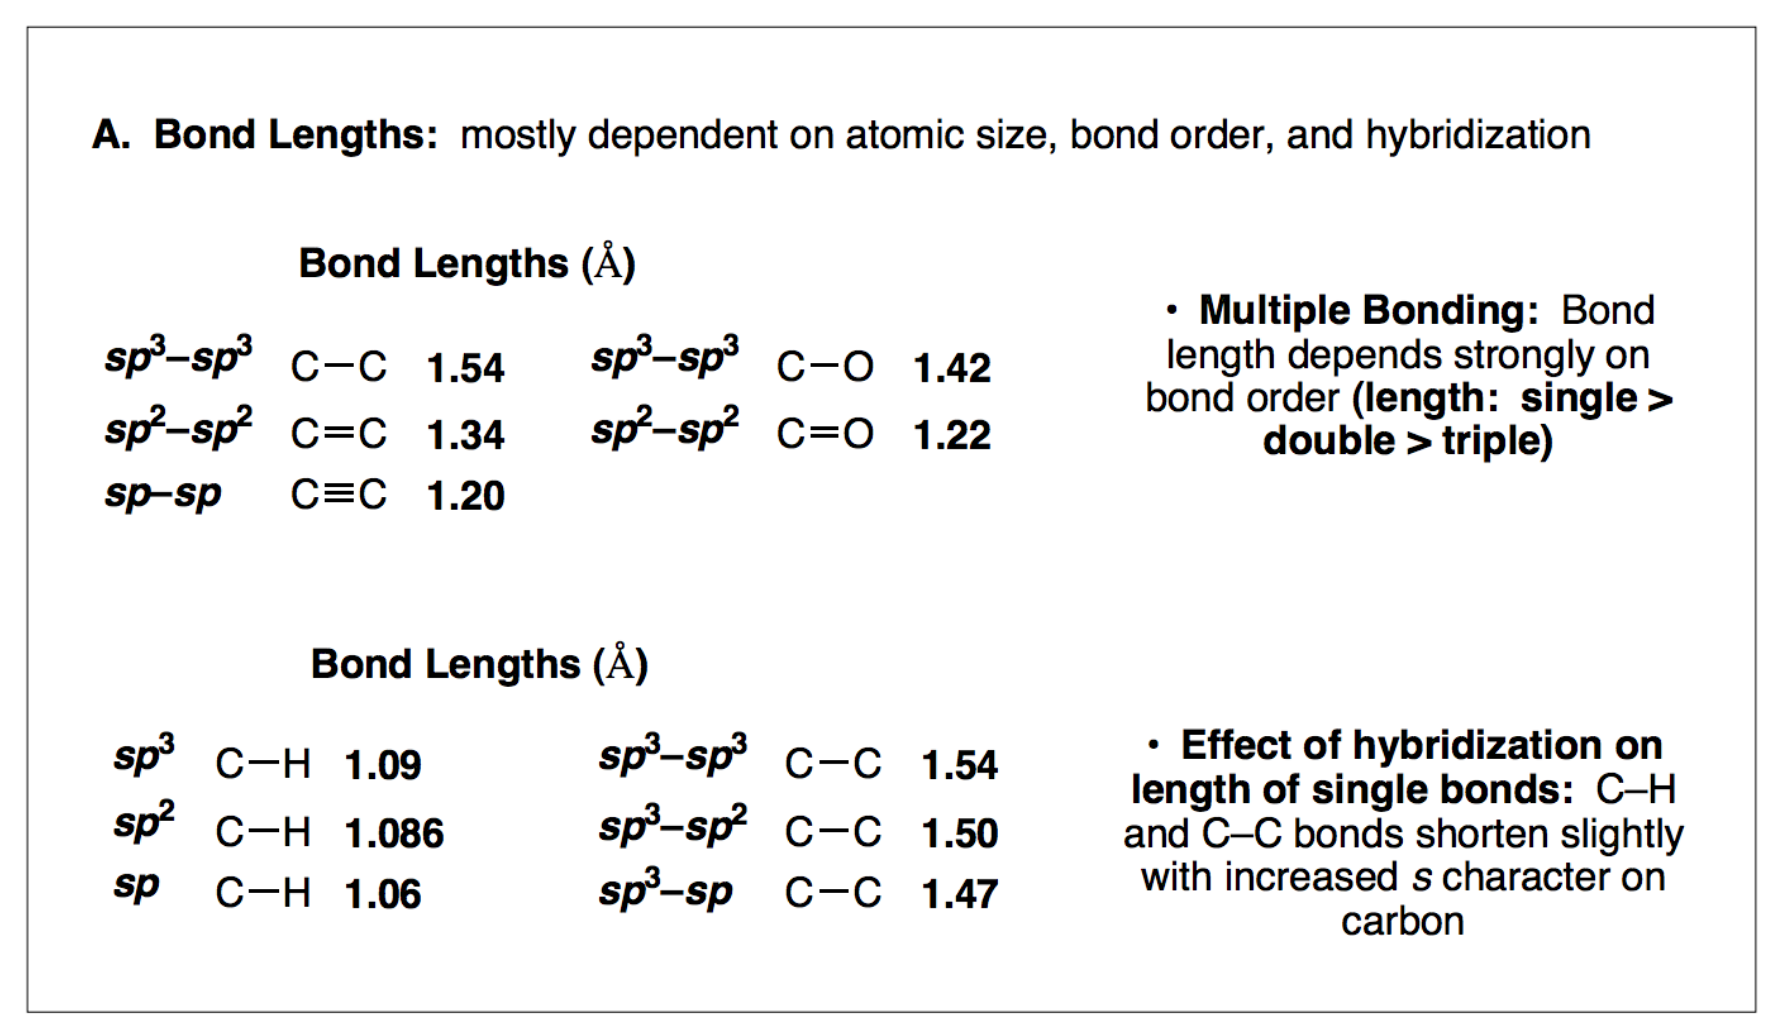
\includegraphics[width = \textwidth]{bond-lengths}\]
\section{General rules of drawing skeletal structures}
\label{sec:orge23bce2}
\begin{enumerate}
\item Carbon atoms aren't usually shown. Instead, a carbon atom is assumed to be at each intersection of two lines (bonds) and at the end of each line.
\item Hydrogen atoms bonded to carbon aren't shown.
\item Atoms other than carbon and hydrogen are shown.
\end{enumerate}

\newpage
\section{Hybridisation in organic molecules}
\label{sec:org3886beb}
Carbon atoms use hybrid orbitals to form bonds in organic molecules.

\begin{itemize}
\item In single bonds with tetrahedral geometry, carbon has 4 \(\boldsymbol{sp^3}\) \textbf{hybrid orbitals}.
\item In double bonds with planar geometry, carbon uses 3 equivalent \(\boldsymbol{sp^2}\) \textbf{hybrid orbitals} and 1 unhybridised \(p\) orbital.
\item Carbon uses 2 equivalent \(\boldsymbol{sp}\) \textbf{hybrid orbitals} to form a triple bond with linear geometry, along with 2 unhybridised \(p\) orbitals.
\end{itemize}

Atoms such as nitrogen and oxygen hybridise to form strong, oriented bonds.

\begin{itemize}
\item The nitrogen atom in ammonia and the oxygen atom in water are \(sp^3\)-hybridised.
\end{itemize}

\[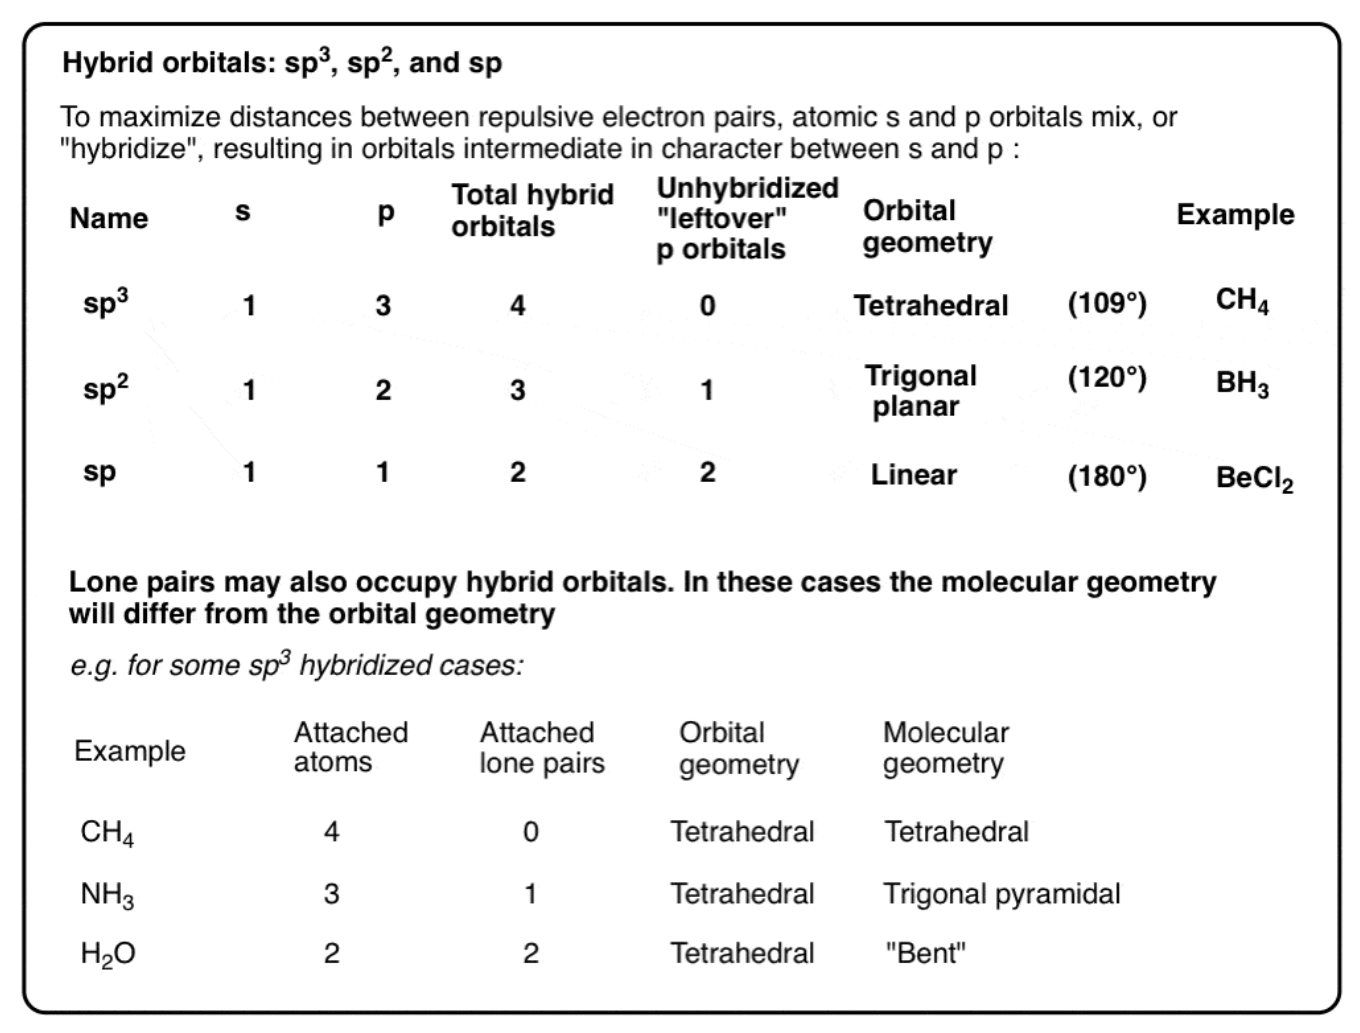
\includegraphics[width = \textwidth]{hybrid-orbitals}\]
\end{document}
